\documentclass[12pt, twoside]{article}
\usepackage[letterpaper, margin=1in, headsep=0.5in]{geometry}
\usepackage[english]{babel}
\usepackage[utf8]{inputenc}
\usepackage{amsmath}
\usepackage{amsfonts}
\usepackage{amssymb}
\usepackage{tikz}
\usetikzlibrary{quotes, angles}
\usepackage{graphicx}
\usepackage{enumitem}
\usepackage{multicol}

\newif\ifmeta
\metatrue %print standards and topics tags

\title{Regents Geometry}
\author{Chris Huson}
\date{January 2022}

\usepackage{fancyhdr}
\pagestyle{fancy}
\fancyhf{}
\renewcommand{\headrulewidth}{0pt} % disable the underline of the header
\raggedbottom

\fancyhead[LE]{\thepage}
\fancyhead[RO]{\thepage \\ Name: \hspace{4cm} \,\\}
\fancyhead[LO]{BECA / Dr. Huson / Geometry 6 Trigonometry}

\begin{document}
\subsubsection*{6.13 Classwork: Tangent variations \hfill CCSS.HSG.SRT.C.8}
For a right triangle, $\displaystyle \tan \theta = \frac{\rm{opposite}}{\rm{adjacent}}$
\begin{enumerate}
\item Do Now: Given right $\triangle JKL$ with $\overline{JK} \perp \overline{KL}$, $JK=10$, $m\angle J=31^\circ$. Let $x$ be the length of the side opposite $\angle J$, $x=KL$.
\begin{enumerate}
  \item Mark up the triangle.
  \item Find $x$.
\end{enumerate}
    \begin{flushright}
        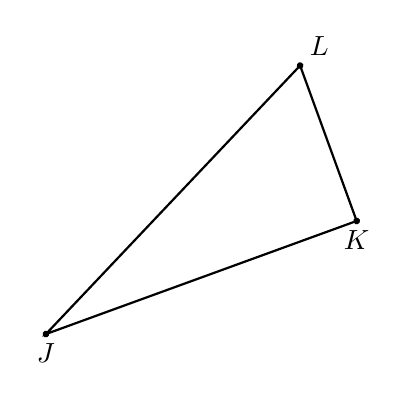
\begin{tikzpicture}[scale=0.7, rotate=20]
          \draw [thick](0,0)--(6,0)--(6,3)--cycle;
          \draw [fill] (0,0) circle [radius=0.05] node[below]{$J$};
          \draw [fill] (6,0) circle [radius=0.05] node[below]{$K$};
          \draw [fill] (6,3) circle [radius=0.05] node[above right]{$L$};
        \end{tikzpicture}
      \end{flushright}

\item $\triangle ABC$ is shown with $m\angle C=90^\circ$ and the lengths of the triangle's sides are $AC=8$, $BC=15$.  \hfill (not drawn to scale)
  \begin{multicols}{2}
    \begin{enumerate}
      \item Write down the value of $\tan A$. \vspace{1.25cm}
      \item Find the measure of $\angle A$. \vspace{1cm}
      \item Write down the value of $\tan B$. \vspace{1.25cm}
      \item Find the measure of $\angle B$ two different ways. \vspace{1cm}
      \item Find $AB$.
    \end{enumerate}
    \begin{flushright}
    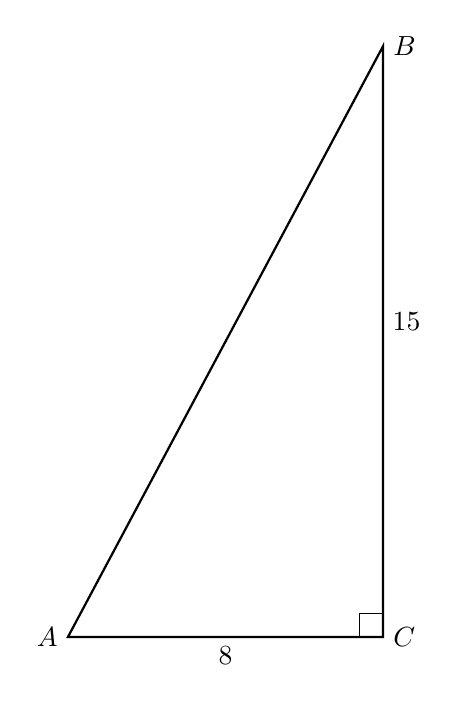
\begin{tikzpicture}[scale=0.5]
      \draw [thick]
      (0,0)node[left]{$A$}--
      (8,0)node[ right]{$C$}--
      (8,15)node[right]{$B$}--cycle;
      \draw (8,0)++(-0.6,0)--++(0,0.6)--+(0.6,0);
      \node at (4,0)[below]{$8$};
      \node at (8,8)[right]{$15$};
      %\node at (2.5,6)[above]{$17$};
    \end{tikzpicture}
    \end{flushright}
  \end{multicols}
  \vspace{3cm}

\newpage
\item Romeo is standing 8 meters away from Juliet's house, looking up at Juliet's window. He is two meters tall and looks up at a $55^\circ$ angle.\\[0.25cm]
Find the height of Juliet's window ledge to the \emph{nearest meter}. \hfill (not drawn to scale)
  \begin{flushright}
    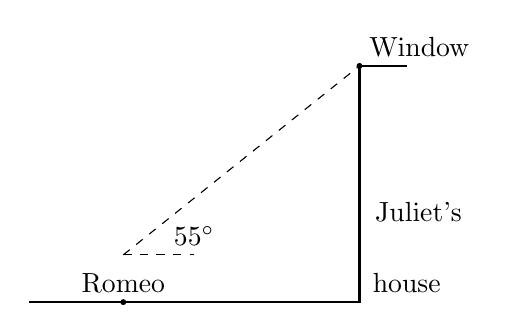
\begin{tikzpicture}[scale=0.3]
      \draw [-, dashed] (0,2)--(3,2);
      \draw [-, thick] (-4,0)--
      (0,0)--
        (10,0)--(10,10)--(12,10);
      \draw [fill] (0,0) circle [radius=0.1] node[above]{Romeo};
      \draw [fill] (10,10) circle [radius=0.1] node[above right]{Window};
      \draw [dashed] (0,2)--(10,10);
      \node at (3, 2)[above]{$55^\circ$};
      \node at (12, 0)[above]{house};
      \node at (12.5, 3)[above]{Juliet's };
    \end{tikzpicture}
    \end{flushright}
    

\item From the top of a lighthouse, a ship is visible at an angle of depression of $3^\circ$. If the lighthouse is 1000 meters tall, determine the distance of the ship from the lighthouse, $x$, to the \emph{nearest kilometer}.
\begin{center}
    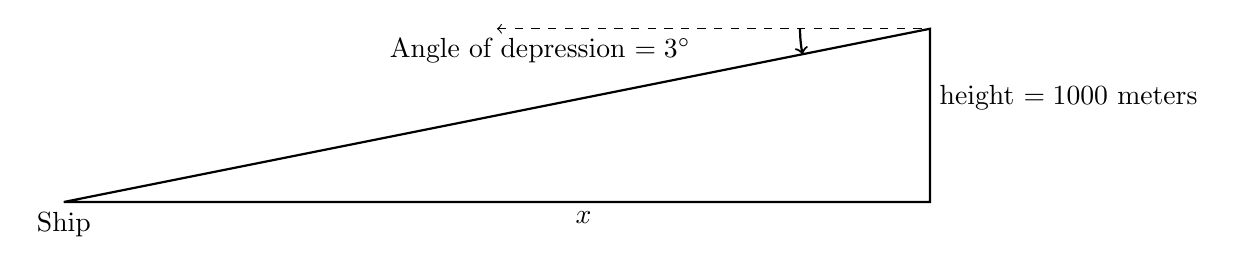
\begin{tikzpicture}[scale=1.1]
      \draw [thick] (10,0)--(0,0)--(10,2.0)--cycle;
      \draw [dashed, <-] (5,2)--(10,2.0);
      \draw [thick, ->] (8.5,2) arc [start angle=180, end angle=191.3, radius=1.5];
      \node at (5.5,2)[below]{Angle of depression $=3^\circ$};
      \node at (10,1.2)[right]{height $=1000$ meters};
      \node at (6,0)[below]{$x$};
      \node at (0,0)[below]{Ship};
    \end{tikzpicture}
  \end{center} \vspace{2cm}

\item An airplane flying at an altitude of 3,000 meters is observed twice. The first time the angle of elevation is $5^\circ$ and exactly one minute later the angle of elevation is $7.5^\circ$. \\[0.25cm]
Find the distance the plane flies over the minute and its speed in kilometers per hour.
\begin{flushright}
  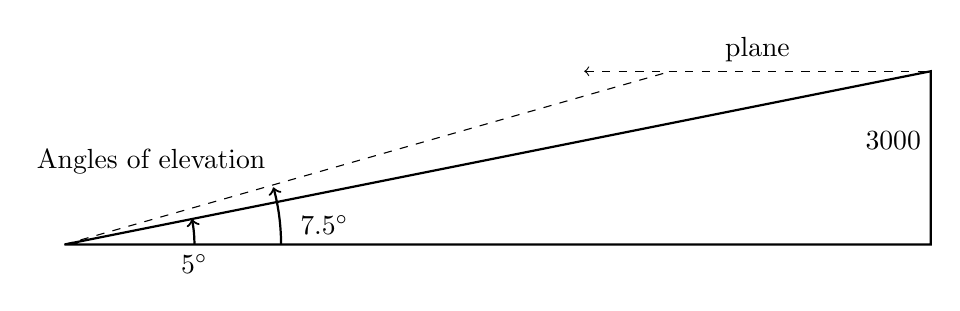
\begin{tikzpicture}[scale=1.1]
    \draw [thick] (10,0)--(0,0)--(10,2.0)--cycle;
    \draw [dashed] (0,0)--(7,2.0);
    \draw [dashed, <-] (6,2)--(10,2);
    \draw [thick, ->] (1.5,0) arc [start angle=0, end angle=11.3, radius=1.5];
    \draw [thick, ->] (2.5,0) arc [start angle=0, end angle=15.3, radius=2.5];
    \node at (1,0.7)[above]{Angles of elevation};
    \node at (1.5,0)[below]{$5^\circ$};
    \node at (3,0)[above]{$7.5^\circ$};
    \node at (10,1.2)[left]{$3000$};
    \node at (8,2)[above]{plane};
  \end{tikzpicture} 
\end{flushright}
\vspace{4cm}

\end{enumerate}
\end{document}